\documentclass[12pt,a4paper]{article}
\usepackage{cmap} % Makes the PDF copiable. See http://tex.stackexchange.com/a/64198/25761
\usepackage[T1]{fontenc}
\usepackage[brazil]{babel}
\usepackage[utf8]{inputenc}
\usepackage{amsmath}
\usepackage{amsfonts}
\usepackage{amssymb}
\usepackage{amsthm}
\usepackage{textcomp} % \degree
\usepackage{gensymb} % \degree
\usepackage[usenames,svgnames,dvipsnames]{xcolor}
\usepackage{hyperref}
\usepackage{multicol}
\usepackage{graphicx}
\usepackage[margin=2cm]{geometry}
\usepackage{icomma} % vírgulas como pontuação vs ponto decimal
\hypersetup{
    colorlinks = true,
    allcolors = {blue}
}

\newcommand{\fixme}{{\color{red}(...)}}
\newcommand*\sen{\operatorname{sen}}
\newcommand*\tg{\operatorname{tg}}
\newcommand*\arctg{\operatorname{arctg}}
\newcommand*\R{\mathbb{R}}
\newcommand*\diff{\mathop{}\!\mathrm{d}}

\newcommand{\IconPc}{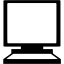
\includegraphics[width=1em]{computer.png}}
\newcommand{\IconCalc}{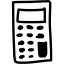
\includegraphics[width=1em]{calculator.png}}
\newcommand{\IconThink}{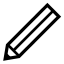
\includegraphics[width=1em]{pencil.png}}
\newcommand{\IconCheck}{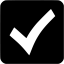
\includegraphics[width=1em]{checkmark.png}}
\newcommand{\IconConcept}{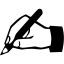
\includegraphics[width=1em]{edit.png}}

\newlength{\SmileysLength}
\setlength{\SmileysLength}{\labelwidth}\addtolength{\SmileysLength}{\labelsep}

\newcommand{\calc}{\hspace*{-\SmileysLength}\makebox[0pt][r]{\IconCalc}%
   \hspace*{\SmileysLength}}
\newcommand{\software}{\hspace*{-\SmileysLength}\makebox[0pt][r]{\IconPc}%
   \hspace*{\SmileysLength}}
\newcommand{\teoria}{\hspace*{-\SmileysLength}\makebox[0pt][r]{\IconThink}%
   \hspace*{\SmileysLength}}
\newcommand{\conceito}{\hspace*{-\SmileysLength}\makebox[0pt][r]{\IconCheck}%
   \hspace*{\SmileysLength}}
\newcommand{\concept}{\hspace*{-\SmileysLength}\makebox[0pt][r]{\IconCheck}%
   \hspace*{\SmileysLength}}

\newcommand*\tipo{Lista de Exercícios - Integração Numérica}
%\newcommand*\turma{...}
\newcommand*\disciplina{ANN0001/CAN0001}
\newcommand*\eu{Helder G. G. de Lima}
\newcommand*\data{\today}

\author{\eu}
\title{\tipo}
\date{\data}

\begin{document}

\begin{center}

\includegraphics[width=9.0cm]{marca} \\
\textbf{\tipo} \\
Prof. \eu\footnote{
Este é um material de acesso livre distribuído sob os termos da licença \href{https://creativecommons.org/licenses/by-sa/4.0/deed.pt_BR}{Creative Commons BY-SA 4.0}.}
\end{center}

%\section*{Legenda}
%\begin{multicols}{4}
%\begin{itemize}
%\item[] \hspace*{\SmileysLength} \calc \hspace*{-\SmileysLength} Cálculos
%\item[] \hspace*{\SmileysLength} \conceito \hspace*{-\SmileysLength} Conceitos
%\item[] \hspace*{\SmileysLength} \teoria \hspace*{-\SmileysLength} Teoria
%\item[] \hspace*{\SmileysLength} \software \hspace*{-\SmileysLength} Software
%\end{itemize}
%\end{multicols}

\section*{Questões}

\begin{enumerate}
\item Uma forma simples de estimar o valor de $\int_a^b f(x)\diff{x}$ é utilizar o \textit{método do ponto médio}, um método de Newton-Cotes aberto, no qual considera-se um retângulo cuja base é o intervalo $[a,b]$ e a altura é o valor de $f$ no ponto médio deste intervalo, ou seja:
\[
\int_a^b f(x)\diff{x} \approx (b-a) \cdot f\left(m \right),
\quad
m = \frac{a+b}{2}.
\]

Calcule numericamente as integrais a seguir por meio de uma única aplicação das regras: (1) do ponto médio, (2) do trapézio, (3) 1/3 de Simpson, (4) 3/8 de Simpson e (5) de Boole. Obtenha também as soluções exatas e compare-as com as aproximações obtidas, calculando os erros relativos percentuais. Interprete geometricamente.
\begin{multicols}{4}
\begin{enumerate}
\item $\int_0^1 3x^2 \diff{x}$
% I = 1
\item $\int_0^1 4x^3 \diff{x}$
% I = 1
\item $\int_{0}^1 x^9 - 3x^2 \diff{x}$
% I = -0.9
\item $\int_{1}^5 \frac{4}{x} - \cos(x) \diff{x}$
% I ≈ 8.2381
\end{enumerate}
\end{multicols}

\item Considere a integral $I = \int_0^2 \cos(x^2)\diff{x}$, cujo valor com 10 casas decimais corretas é $0.4614614624$. Subdivida o intervalo $[a, b] = [0, 2]$ utilizando $n+1$ pontos igualmente espaçados, $a = x_0 < x_1 < \ldots < x_n = b$, e calcule numericamente o valor aproximado de $I$ aplicando repetidas vezes os métodos do ponto médio, do trapézio e 1/3 de Simpson aos subintervalos $[x_i,x_{i+1}]$. Compare os resultados obtidos com $n = 1, 2, 4, 8$.

\item Seja $M$ a aproximação de $\int_a^b f(x)\diff{x}$ fornecida pela regra do ponto médio, $T$ a aproximação obtida pela regra do trapézio e $S$ a aproximação que resulta da regra 1/3 de Simpson. Mostre que $S$ é uma média aritmética ponderada de $M$ e $T$.

\item Qual é o maior valor de $h \in \mathbb{R}$ para o qual a regra do trapézio aproxima $\int_0^h f(x) \diff{x}$ com um erro absoluto $|\varepsilon_{abs}| \leq 0,1$ considerando que $f(x) = x^2$? E se $f(x) = x^3$, o valor de $h$ aumenta, diminui ou permanece o mesmo? O que se pode esperar de outras funções $f(x) = x^n$, com $n = 4,5,6,\ldots$? Explique.

\item Considere uma função $g$ que assume os valores dados na tabela a seguir:
%g(x) = (x² + 1) cos(x π / 12 )
\begin{center}
\begin{tabular}{|c|c|c|c|c|c|c|c|}
\hline
   $x_i$ & 0 & 1 & 2 & 3 & 4 & 5 & 6 \\ \hline
$g(x_i)$ & 1.00 & 1.93 & 4.33 & 7.07 & 8.50 & 6.73 & 0.00 \\
\hline
\end{tabular}
\end{center}
Estime $\int_0^6 g(x)\diff{x}$ utilizando os métodos a seguir no maior número de subintervalos de mesmo comprimento que for possível:
\begin{multicols}{2}
\begin{enumerate}
\item A regra do trapézio.
\item A regra 1/3 de Simpson.
\end{enumerate}
\end{multicols}

\item Explique uma das regras de integração/quadratura numéricas, e deduza a fórmula correspondente a partir de sua interpretação geométrica.

\item Durante os primeiros segundos após o lançamento de um foguete em direção à lua, foi registrado que sua velocidade aumentava conforme a tabela a seguir:
\begin{center}
\begin{tabular}{|c|c|c|c|c|c|c|c|}
\hline
  $t\ (s)$ & 0 & 10 & 20 & 30 & 40 \\ \hline
$v\ (m/s)$ & 0 & 65,5 & 180,7 & 345,7 & 560,2 \\
\hline
\end{tabular}
\end{center}
Calcule a altura do foguete após 40 segundos utilizando a regra 1/3 de Simpson.

\item Estime as integrais a seguir utilizando a quadratura de Gauss-Legendre com 2 a 5 pontos, depois de realizar uma mudança de variáveis apropriada para usar o intervalo $[-1,1]$:
\begin{multicols}{4}
\begin{enumerate}
\item $\int_0^2 x^2 + x\diff{x}$
\item $\int_1^2 \frac{2}{x^2}\diff{x}$
\item $\int_{-1}^3 e^{-x^2}\diff{x}$
\item $\int_{-3}^3 \frac{1}{1+x^2} \diff{x}$
\end{enumerate}
\end{multicols}

\item Utilize o método de Romberg para estimar o valor de $\pi = \int_{-1}^1 \frac{2}{x^2 + 1}\diff{x}$, com um erro relativo percentual inferior a $0,1\%$.

\item Forneça uma estimativa de $\int_1^{1.8} e^x\diff{x}$ com erro relativo menor ou igual a $10^{-7}$, utilizando o esquema de Romberg.

\item Utilize o método de Newton-Cotes adaptável estimar as integrais a seguir:
\begin{enumerate}
\item $\int_{0.3}^{1.5} \tg(x)\diff{x}$, com $|\varepsilon_{rel}| \leq 0.1$, usando 3 dígitos após a vírgula
\item $\int_{0.4}^{2} \ln{x}\diff{x}$, com $|\varepsilon_{rel}| \leq 0.005$, usando 4 dígitos após a vírgula
\item $\int_{1}^{13} \sqrt{x}\diff{x}$, com $|\varepsilon_{rel}| \leq 0.001$, usando 4 dígitos após a vírgula
\item $\int_1^5 \frac{x+1}{x^2}\diff{x}$, com $|\varepsilon_{rel}| \leq 0.02$, usando 3 dígitos após a vírgula
\item $\int_{0.2}^{1} \sen(1/x)\diff{x}$, com $|\varepsilon_{rel}| \leq 0.01$, usando 3 dígitos após a vírgula
\item $\int_{0}^{2} f(x)\diff{x}$, com $|\varepsilon_{rel}| \leq 0.01$, considerando que $f(x)$ assume os seguintes valores:
%f(x) = cos(3x) + 21 / (7 + x⁸)
\begin{center}\hspace{-1cm}
\begin{tabular}{|c|c||c|c||c|c||c|c||c|c|}
\hline
$x$ & $f(x)$ & $x$ & $f(x)$ & $x$ & $f(x)$ & $x$ & $f(x)$ & $x$ & $f(x)$\\
\hline
0 & 4 & 0.5 & 3.06906 & 1 & 1.63501 & 1.5 & 0.43281 & 2 & 1.04002\\
\hline
0.125 & 3.93051 & 0.625 & 2.69052 & 1.125 & 1.22244 & 1.625 & 0.53945 & 2.125 & 1.04546\\
\hline
0.25 & 3.73168 & 0.75 & 2.32953 & 1.25 & 0.79975 & 1.75 & 0.73322 & 2.25 & 0.92464\\
\hline
0.375 & 3.43101 & 0.875 & 1.99012 & 1.375 & 0.50766 & 1.875 & 0.92255 & 2.375 & 0.68671\\
\hline
\end{tabular}
\end{center}
\end{enumerate}
\end{enumerate}


\newpage
\section*{Algumas respostas}

\begin{enumerate}
\item
\begin{enumerate}
\item A solução exata é $\int_0^1 3x^2 \diff{x} = x^3 \Big|_0^1 = 1$ e as aproximações são:
\begin{center}
\begin{tabular}{crr}
\hline
Método         & Aproximação & Erro percentual \\ \hline
Ponto médio    & $0,75$ & $25\%$ \\
Trapézio       & $1,5$ & $50\%$ \\
1/3 de Simpson & $1$ & $0\%$ \\
3/8 de Simpson & $1$ & $0\%$ \\
Boole          & $1$ & $0\%$ \\
\hline
\end{tabular}
\end{center}
\item A solução exata é $\int_0^1 4x^3 \diff{x} = x^4 \Big|_0^1 = 1$
\begin{center}
\begin{tabular}{crr}
\hline
Método         & Aproximação & Erro percentual \\ \hline
Ponto médio    & $0,5$ & $50\%$ \\
Trapézio       & $2$ & $100\%$ \\
1/3 de Simpson & $1$ & $0\%$ \\
3/8 de Simpson & $1$ & $0\%$ \\
Boole          & $1$ & $0\%$ \\
\hline
\end{tabular}
\end{center}
\item A solução exata é $\int_0^1 x^9 - 3x^2 \diff{x}= \left(\frac{1}{10}x^{10} - x^3\right) \Big|_0^1 = -0,9$
\begin{center}
\begin{tabular}{crr}
\hline
Método         & Aproximação & Erro percentual \\ \hline
Ponto médio    & $-0,748$ &  $16,8837\%$  \\
Trapézio       & $-1$ & $11,1111\%$ \\
1/3 de Simpson & $-0,832$ & $7,5521\%$ \\
3/8 de Simpson & $-0,865$ & $3,864\%$ \\
Boole          & $-0,895$ & $-0,556\%$\\
\hline
\end{tabular}
\end{center}
\item A solução exata é $\int_1^5 \frac{4}{x} - \cos(x) \diff{x} = \left( 4\ln(x) - \sen(x)\right) \Big|_1^5 = 4\ln(5) + \sen(1) - \sen(5) \approx 8,2381$
\begin{center}
\begin{tabular}{crr}
\hline
Método         & Aproximação & Erro percentual \\ \hline
Ponto médio    & $9,2933$ &  $12,8082\%$  \\
Trapézio       & $7,9521$ & $3,4726\%$ \\
1/3 de Simpson & $8,8462$ & $7,3813\%$ \\
3/8 de Simpson & $8,53$ & $3,541\%$ \\
Boole          & $8,264$ & $0,314\%$ \\
\hline
\end{tabular}
\end{center}
\end{enumerate}
\item $\int_0^2 \cos(x^2)\diff{x} \approx 0.4614614624$
\begin{center}
\begin{tabular}{ccccc}
\hline
              & $n=1$     & $n=2$    & $n=4$   & $n=8$ \\ \hline
Ponto médio   & $1.08060$ & $\textbf{0}.34074$ & $\textbf{0.4}2770$ & $\textbf{0.4}5342$ \\
Trapézio      & $\textbf{0}.34636$ & $\textbf{0}.71348$ & $\textbf{0}.52711$ & $\textbf{0.4}7740$ \\
Simpson (1/3) & $\textbf{0}.83586$ & $\textbf{0.46}499$ & $\textbf{0.46}083$ & $\textbf{0.4614}2$ \\
Simpson (3/8) & $\textbf{0}.60960$ & $\textbf{0.46}211$ & $\textbf{0.461}18$ & $\textbf{0.4614}4$ \\
\hline
\end{tabular}
\end{center}
\item A aproximação $S$ de $\int_a^b f(x)\diff{x}$ que resulta da regra 1/3 de Simpson é dada por:
\begin{align*}
S
& = \frac{\left(\frac{b - a}{2}\right)}{3}\left[ f(a) + 4\cdot f\left(\frac{a + b}{2}\right) + f(b) \right] \\
& = \frac{b - a}{6} \left[ 4\cdot f\left(\frac{a + b}{2}\right) + f(a) + f(b) \right] \\
& = \frac{2}{3} \cdot \left[ (b - a) \cdot f\left(\frac{a + b}{2}\right)\right]
    + \frac{1}{3} \left[ \frac{b - a}{2} \left(f(a) + f(b) \right)\right] \\
& = \frac{2}{3} \cdot M + \frac{1}{3} T,
\end{align*}
em que $M = (b - a) \cdot f\left(\frac{a + b}{2}\right)$ é a aproximação pela regra do ponto médio e $T = \frac{b - a}{2} \left(f(a) + f(b) \right)$ é a aproximação pela regra do trapézio. Portanto, $S$ é uma média ponderada de $M$ e $T$ com pesos $2/3$ e $1/3$, respectivamente.

\item Para $f(x) = x^2$, tem-se $h_{max}=\sqrt[3]{6} \approx 1,8$. Para $f(x) = x^3$, tem-se $h_{max}=\sqrt[4]{4}\approx 1,4 < 1,8$. Em geral, para $f(x) = x^n$, $h_{max}=\sqrt[n+1]{\frac{2n+2}{n-1}}$ diminui conforme $n$ aumenta.
\item
\begin{enumerate}
\item $\int_0^6 g(x)\diff{x} \approx 29.0623$, aplicando a regra do trapézio em $6$ subintervalos
\item $\int_0^6 g(x)\diff{x} \approx 29.8630$, aplicando a regra 1/3 de Simpson em $3$ subintervalos
\end{enumerate}
\item \begin{itemize}
\item \textbf{Regra dos trapézios}: Pode ser deduzida interpolando a função $f$ por um polinômio de grau menor ou igual a $1$ nas extremidades $a$ e $b$ do intervalo de integração, e integrando esse polinômio interpolador.
\item \textbf{Regra de 1/3 de Simpson}: Pode ser deduzida interpolando a função $f$ por um polinômio de grau menor ou igual a $2$ nas extremidades $a$ e $b$ do intervalo de integração, e em seu ponto médio, e integrando esse polinômio interpolador.
\item \textbf{Regra de 3/8 de Simpson}: Pode ser deduzida interpolando a função $f$ por um polinômio de grau menor ou igual a $3$ em quatro pontos igualmente espaçados, incluindo as extremidades $a$ e $b$ do intervalo de integração, e integrando esse polinômio interpolador.
\item \textbf{Quadratura Gaussiana com 2 pontos}: Pode ser deduzida interpolando a função $f$ por um polinômio de grau menor ou igual a $1$ em nós $x_0$ e $x_1$ pertencentes ao intervalo $[a, b]$, escolhidos de modo a obter uma regra de quadratura $I = w_0x_0 + w_1 x_1$ que seja exata para polinômios $p(x) = x^k$, para cada $k=0,\ldots, 3$.
\end{itemize}
\item A altura é de aproximadamente $8554,67$ metros.
\item
\begin{enumerate}
\item $\int_0^2 x^2 + x\diff{x} = \left( \frac{1}{3}x^3 +\frac{1}{2}x^2 \right)\Big|_0^2 = 14/3 \approx 4.6667$
\begin{center}
\begin{tabular}{crr}
\hline
Pontos & Aproximação \\ \hline
2      & $4,666666$ \\
3      & $4,666670$ \\
4      & $4,666666$ \\
5      & $4,666669$ \\
\hline
\end{tabular}
\end{center}
\item $\int_1^2 \frac{2}{x^2}\diff{x} = \left( \frac{-2}{x} \right)\Big|_1^2 = 1$
\begin{center}
\begin{tabular}{crr}
\hline
Pontos & Aproximação \\ \hline
2      & $0,994083$ \\
3      & $0,999749$ \\
4      & $0,999990$ \\
5      & $1,000000$ \\
\hline
\end{tabular}
\end{center}
\item $\int_{-1}^3 e^{-x^2}\diff{x} \approx 1.63303$
\begin{center}
\begin{tabular}{crr}
\hline
Pontos & Aproximação \\ \hline
2      & $1,971967$ \\
3      & $1,477486$ \\
4      & $1,668221$ \\
5      & $1,628089$ \\
\hline
\end{tabular}
\end{center}
\item O valor exato é $\int_{-3}^3 \frac{1}{1+x^2} \diff{x} = \arctg(x) \Big|_{-3}^3 = 2 \arctg(3) \approx 2.49809154479651$.
\begin{center}
\begin{tabular}{crr}
\hline
Pontos & Aproximação \\ \hline
2      & $1,500001$ \\
3      & $3,187500$ \\
4      & $2,189781$ \\
5      & $2,671700$ \\
\hline
\end{tabular}
\end{center}
\end{enumerate}
\item $\pi \approx R_{5,5} \approx 3.141582321$
\item $\int_1^{1.8} e^x\diff{x}
= \left(e^x \right)\Big|_{1}^{1.8}
= e^{1.8} - e
\approx R_{5,5}
\approx 3.331365637$.
\item \begin{enumerate}
\item \begin{itemize}
   \item Valor exato: $\int_{0.3}^{1,5} \tg(x)\diff{x} = -\ln(\cos(1,5))+\ln(\cos(0,3)) \approx 2,603$
   \item Newton-Cotes adaptável: \fixme
\end{itemize}
\item \begin{itemize}
   \item Valor exato: $\int_{0,4}^{2} \ln{x}\diff{x} = (2 \ln(2) - 2)-(0,4 \ln(0,4) - 0,4) \approx 0,1528$
   \item Newton-Cotes adaptável: \fixme
\end{itemize}
\item \begin{itemize}
   \item Valor exato: $\int_{1}^{13} \sqrt{x}\diff{x} = \frac{2}{3}(13 \sqrt{13} - 1) \approx 30,5814$
   \item Newton-Cotes adaptável: \fixme
\end{itemize}
\item \begin{itemize}
   \item Valor exato: $\int_1^5 \frac{x+1}{x^2}\diff{x} = \frac{4}{5} + \ln(5) \approx 2,409$
   \item Newton-Cotes adaptável: \fixme
\end{itemize}
\item \begin{itemize}
   \item Valor exato: $\int_{0,2}^{1} \sen(1/x)\diff{x} \approx 0,506$
   \item Newton-Cotes adaptável: \fixme
\end{itemize}
\item \begin{itemize}
   \item Valor exato: $\int_{0}^{2} f(x)\diff{x} \approx 3,80997$
   \item Newton-Cotes adaptável: \fixme
\end{itemize}
\end{enumerate}
\end{enumerate}
\end{document}
